%
% File naaclhlt2018.tex
%
%% Based on the style files for NAACL-HLT 2018, which were
%% Based on the style files for ACL-2015, with some improvements
%%  taken from the NAACL-2016 style
%% Based on the style files for ACL-2014, which were, in turn,
%% based on ACL-2013, ACL-2012, ACL-2011, ACL-2010, ACL-IJCNLP-2009,
%% EACL-2009, IJCNLP-2008...
%% Based on the style files for EACL 2006 by 
%%e.agirre@ehu.es or Sergi.Balari@uab.es
%% and that of ACL 08 by Joakim Nivre and Noah Smith

\documentclass[11pt,a4paper]{article}
\usepackage[hyperref]{naaclhlt2018}
\usepackage{times}
\usepackage{latexsym}
\usepackage{amsfonts}
\usepackage{booktabs}
\usepackage{siunitx}
\usepackage{graphicx}

\usepackage{url}

\aclfinalcopy % Uncomment this line for all SemEval submissions

%\setlength\titlebox{5cm}
% You can expand the titlebox if you need extra space
% to show all the authors. Please do not make the titlebox
% smaller than 5cm (the original size); we will check this
% in the camera-ready version and ask you to change it back.

\newcommand\BibTeX{B{\sc ib}\TeX}

%Title format for system description papers by task participants
\title{UAIC at SemEval-2019 Task 3: Extracting Much from Little}
%Title format for task description papers by task organizers
%\title{SemEval-2018 Task [TaskNumber]:  [Task Name]}


{
\addtolength{\oddsidemargin}{-.875in}
\addtolength{\evensidemargin}{-.875in}
\addtolength{\textwidth}{1.75in}

\author{Cristian Simionescu, Ingrid Stoleru, Diana Lucaci, Gheorghe Balan, \\ \textbf{Iulian Bute, Adrian Iftene}\\\\
  Faculty of Computer Science, "Alexandru Ioan Cuza" University of Iasi, Romania\\
  {\tt cristian@nexusmedia.ro, ingridstoleru@gmail.com, \\
  {\tt \{diana.lucaci22, balangheorghe1997\}@gmail.com,\\
  {\tt iulian.bute@gmail.com, adiftene@info.uaic.ro}}}}


\date{23 February 2019}
}
\begin{document}

\maketitle

\begin{abstract}
In this paper, we present a system description for implementing a sentiment analysis agent capable of interpreting the state of an interlocutor engaged in short three message conversations. We present the results and observations of our work and which parts could be further improved in the future. 
\end{abstract}

\section{Introduction}

It is hard to understand emotions in textual conversations in the absence of voice modulations and facial expressions \cite{Gupta2017ASA}. In sentiment analysis task researchers work on different levels of sentiment analysis: document (when are considered single topics documents), sentence (when single sentences are classified as positive, negative or neutral), entity or aspect (which deal with finding the aspects in the text and then classifying in respective aspect) \cite{Liu12}. 

Similar to sentiment analysis at sentence level, in last years tweets from Twitter were analyzed and classified \cite{Zhang2017}, \cite{kumar12}, \cite{Mukherjee2013} and \cite{kumar14}. In the beginning, a binary classification was used, which linked opinions or opinions only to two classes: positive or negative. In \cite{Pak2010TwitterAA} the authors proposed a model for classifying tweets in goals, positive and negative feelings using a classifier based on multinomial Naive Bayes to use features such as N-grams and tags POS (part- of-Speech). In \cite{Parikh} the authors have implemented two models, one based on the Naive Bayes bigrams model and one using Maximum Entropy to classify tweets. \cite{Go_Bhayani_Huang_2009} proposed a solution for analysing feelings on Twitter using distant supervision, the training data were tweets with emoticons, which are regarded as noise data. They built several well performing models using Naive Bayes, MaxEnt, and SVM. \cite{barbosa2010} have modeled an automated method to classify tweets using space features including retweets, hashtags, links, punctuation mark amazement in combination with words and POS features polarity. \cite{Luo2013} have brought to light the difficulties that they encounter when they want to classify tweets. Spam and a variety of languages on Twitter make the task of identifying opinions very difficult.

In SemEval 2019, in Task 3, EmoContext: Contextual Emotion Detection in Text \cite{SemEval2019Task3}, the organizers ask participants to classify users’ messages in one of four classes: {\textit{Happy}}, {\textit{Sad}}, {\textit{Angry}} or {\textit{Others}}. These are given in the context of another two previous messages. The textual dialogue is composed of short messages that appear to be from a chat conversation. In such a context, the users express their thoughts and ideas in a compact way. In this paper, we describe how we created one classifier to detect the sentiment of short messages such as tweets. 
\section{Related Work}

\subsection{Word Embeddings}
In order to incorporate the meaning of the words in a software system that processes natural language, distributed representations of words in a vector space are used to achieve better results by grouping similar words. 

Previous work ~\cite{mikolov:13} introduces two architectures {\textit{CBOW}} (Continuous Bag-of-Words) and {\textit{Skip-gram model}} for learning word representations using neural networks. The later is more efficient for small training data, generating better representations for the infrequent words ~\cite{study:17}.

When choosing the best representations for a certain training dataset, one can either use pre-trained word embeddings that were built using large general corpora or train their own embeddings on a specific corpus which is similar to the type of data the model will be working with. The advantage of the first approach is that the representations only need to add without any additional computational cost, meanwhile, the second one requires a large enough corpus that can lead to meaningful representations that can capture both syntactic and semantic regularities. While vectors like Word2Vec, GloVe (Global Vectors for Word Representation) or fastText capture the most frequent semantic meaning of the words, training new representation on social media data can bring a number of advantages such as embedding the specific informal language that is used on these platforms and comprising numerous words that might not be very frequent in general corpora ~\cite{Rotari2017} and ~\cite{Flescan2017}.

\section{System Architecture}

In this section we will present the systems developed for the EmoContext task.

\subsection{Data Pipeline}

Starting off, a critical characteristic in our architecture was the ease of configuration of different parameters of our system. We want our system to require little additional work and troubleshooting when changing, adding or removing pre-processing, feature extractions or post-processing techniques.

As seen in Figure \ref{fig:pipeline1}, the system can take any configuration and order of pre-processing, feature extraction and post-process methods as well as a model to be fed the data.

\begin{figure}[h]
    \centering
    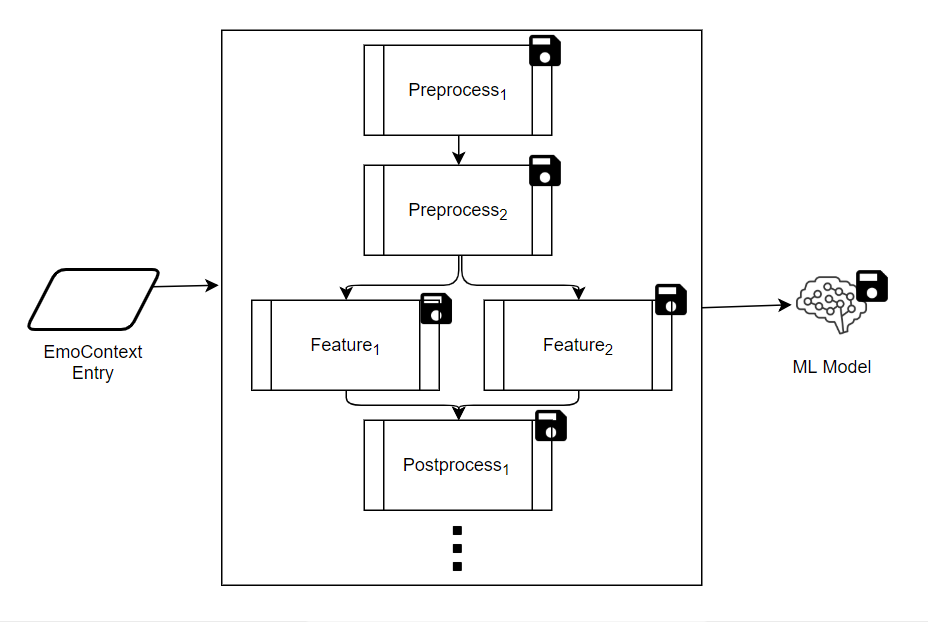
\includegraphics[width=0.5\textwidth]{images/pipeline_figure.PNG}
    \caption{Pipeline structure}
    \label{fig:pipeline1}
\end{figure}

Since a lot of small changes would sometimes occur on the later stages of the pipeline, we implemented an auto-save feature in all components of the system which will simply use the cached processed data up to the point of the last modified step in the pipeline.

\subsection{Data Processing}

The dataset in from EmoContext task presented some clear challenges. Since we had to learn the expected sentiment of one of the interlocutors from a relatively small amount of text it was of utmost importance to remove noise from the data with minimal loss of potentially useful information. With such small amount of data ($\approx$ 4 words per message) in each column, we decided to concatenate all three messages in every entry in order to be able to infer more information from it.

\subsection{Pre-processing Stage}

In the pre-processing stage, we implemented a number of steps progressively remove noise such as non utf-8 encoded symbols or random punctuation or characters, from which no important information could be extracted, using regex rewriting rules. After which we transform all misspelled words to the closest correct English word (closest in terms of Hamming distance) while some words would be transformed wrongly, the system performed better when using the "corrected" dataset.

We considered emoticons to be important in determining the sentiment state of the communicating parties, as such we identified as many standard use emoticons. With these emoticons, we analyzed the distribution of where they appear. For example: ":)" appeared predominantly in entries labeled "happy". Using these we replaced each emoticon with the keywords: "happyemoticon", "angryemoticon", "angryemoticon" and "otheremoticon" respectively.

In terms of the actual noise reducing rewriting rules:
\begin{itemize}
    \item Eliminating any elongated series of characters greater than two, to a size of two;
    \item Reducing any repetition of English symbols or punctuation marks to just one, since it would not lead to any loss of information but it will remove noise;
    \item Removal of spaces between punctuation marks;
    \item Removal of any number with more than one decimal;
    \item Rewriting Unicode characters into utf-8 equivalents or complete removals when not possible;
    \item Isolated characters get deleted;
    \item Deletion of ASCII emoticons.
\end{itemize}

We have observed that this combination of pre-processes leads to the best results, without eliminating too much or leaving too much noise. Extensive empirical experimentation was done to assert the performance of various combinations of pre-processes and parameters.

We have to keep in mind, that before applying these modifications the average length of the concatenated messages is around 12 words, afterward, it became around 10. 

\subsection{Feature Selection}

For the actual features we wanted to use in our system, we have attempted a number of syntactic features we thought of extracting. 

All of these features proved to be either not helpful in the aid of the model performance or detrimental in the sense that it left any model we attempted prone to overfitting, such as getting stuck in the local maxima of classifying all instances as "others".

As such, we chose to use embeddings as our only form of feature selection. We have tried to utilize pre-trained embeddings offered online such as GloVe, FastText and Word2vec. 

Sadly, all of the embeddings we have attempted to incorporate into the system produced weaker results compared to training the embedding from scratch on the data.

For this, we tokenized the data and padded it to have 200 elements per list. Even though these vectors were trained on a relatively small corpus, due to the high usage of jargon, rare abbreviations and bad grammar which made our dataset very much different compared to the corpus used by any of the above mentioned pre-trained word embeddings this was most likely the cause of improved performance when our own embedding even though the corpus is extremely small compared to what would be required to create a good embedding. 

\subsection{Model}

In constructing our machine learning model, we chose to use artificial neural networks with the use of the "Keras" python library\footnote{https://keras.io/}.

For the actual model of the system, we have made use of very simple and small architectures since any attempt of creating a deeper or wider artificial neural network models resulted in drastic overfitting. Even with other overfitting alleviating techniques such as regularization, dropout and batch normalization we had to stick to a shallow architecture. We suspect this is due to the fact that we trained our embedding on such a small dataset, perhaps if more similar data can be collected and a more general word vector is created, overfitting would also be reduced. As such, the model we are presenting does not suffer from overfitting but it is relatively shallow. 

\begin{figure}[h]
    \centering
    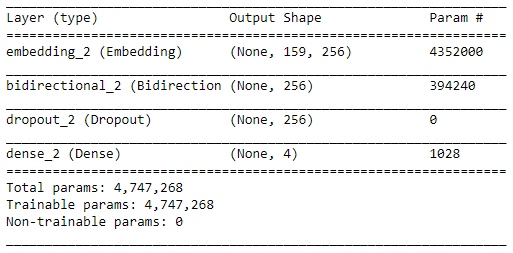
\includegraphics[width=0.48\textwidth]{images/model.png}
    \caption{Model}
    \label{fig:model}
\end{figure}

As seen in Figure \ref{fig:model}, we used a trainable embedding layer of size 256 as input to fit on our training data. Next we used a single hidden layer of 128 Bidirectional LSTM cells with a 30\% dropout and a tanh activation function. Finally outputting the result in a 4 neuron layer using the softmax function to learn the correct expected labels.

The model was trained using the RMSprop optimization algorithm.

\section{Results}

\begin{table*}[h]
  \centering
  \begin{tabular}{l c c c c c}
    \toprule
    \multirow{ } & \multicolumn{3}{c}{Metrics} \\ 
    \cmidrule{2-6}
    & micro F1 & Accuracy & Precision & Recall & Sensitivity \\ 
    \midrule
    Others & \textbf{0.92459089} & 0.87620258 & \textbf{0.95740783} & \textbf{0.89394911} & 0.77644231 \\

    Angry & 0.61855670 & 0.94626974 & 0.50209205 & 0.80536913 & 0.95432738\\

    Sad & 0.63508772 & \textbf{0.96224360} & 0.56562500 & 0.72400000 & 0.97356912 \\ 
    
    Happy & 0.56877323 & 0.95788709 & 0.60236220 & 0.53873239 & \textbf{0.98066986} \\
    
    \textit{Average} & \textit{0.68675210} & \textit{0.93565070} & \textit{0.65687170} & \textit{0.74051260} & \textit{0.92125210} \\
    \bottomrule
  \end{tabular}
    \caption{Submission metrics}
    \label{tab:submission_metrics}
\end{table*}

Using that simple model and an extensive meta-parameter tuning we were able to reach an average micro F1 score of 0.6895, this being the last submission we were able to upload during the workshop. See Table \ref{tab:submission_metrics} for complete metrics of this submission, calculated by training the model 5 times, to factor in for randomness of shuffled data and weight initialization (all runs had comparably similar results).

We noticed that the greatest difficulty our system faces is correctly classifying instances belonging to the "happy" class. As such, we should look into what data pre-processing we could use in order to decrease the high number of false-negatives.

Another potential improvement would be to add weights to the loss function based on the proficiency we observe the system to exhibit on each type of entry.

Applying the pre-processing we described previously we managed to boost that result to average micro F1 of 0.7362.

Both of these models were trained using a K-fold cross-validation with four splits and a batch size of 64.

What we observed time and time again, the main issue we faced was overfitting of the training data, as we can see when looking at the progression on the validation data, see Figure \ref{fig:train_validation_f1}.

\begin{figure}[!h]
    \centering
    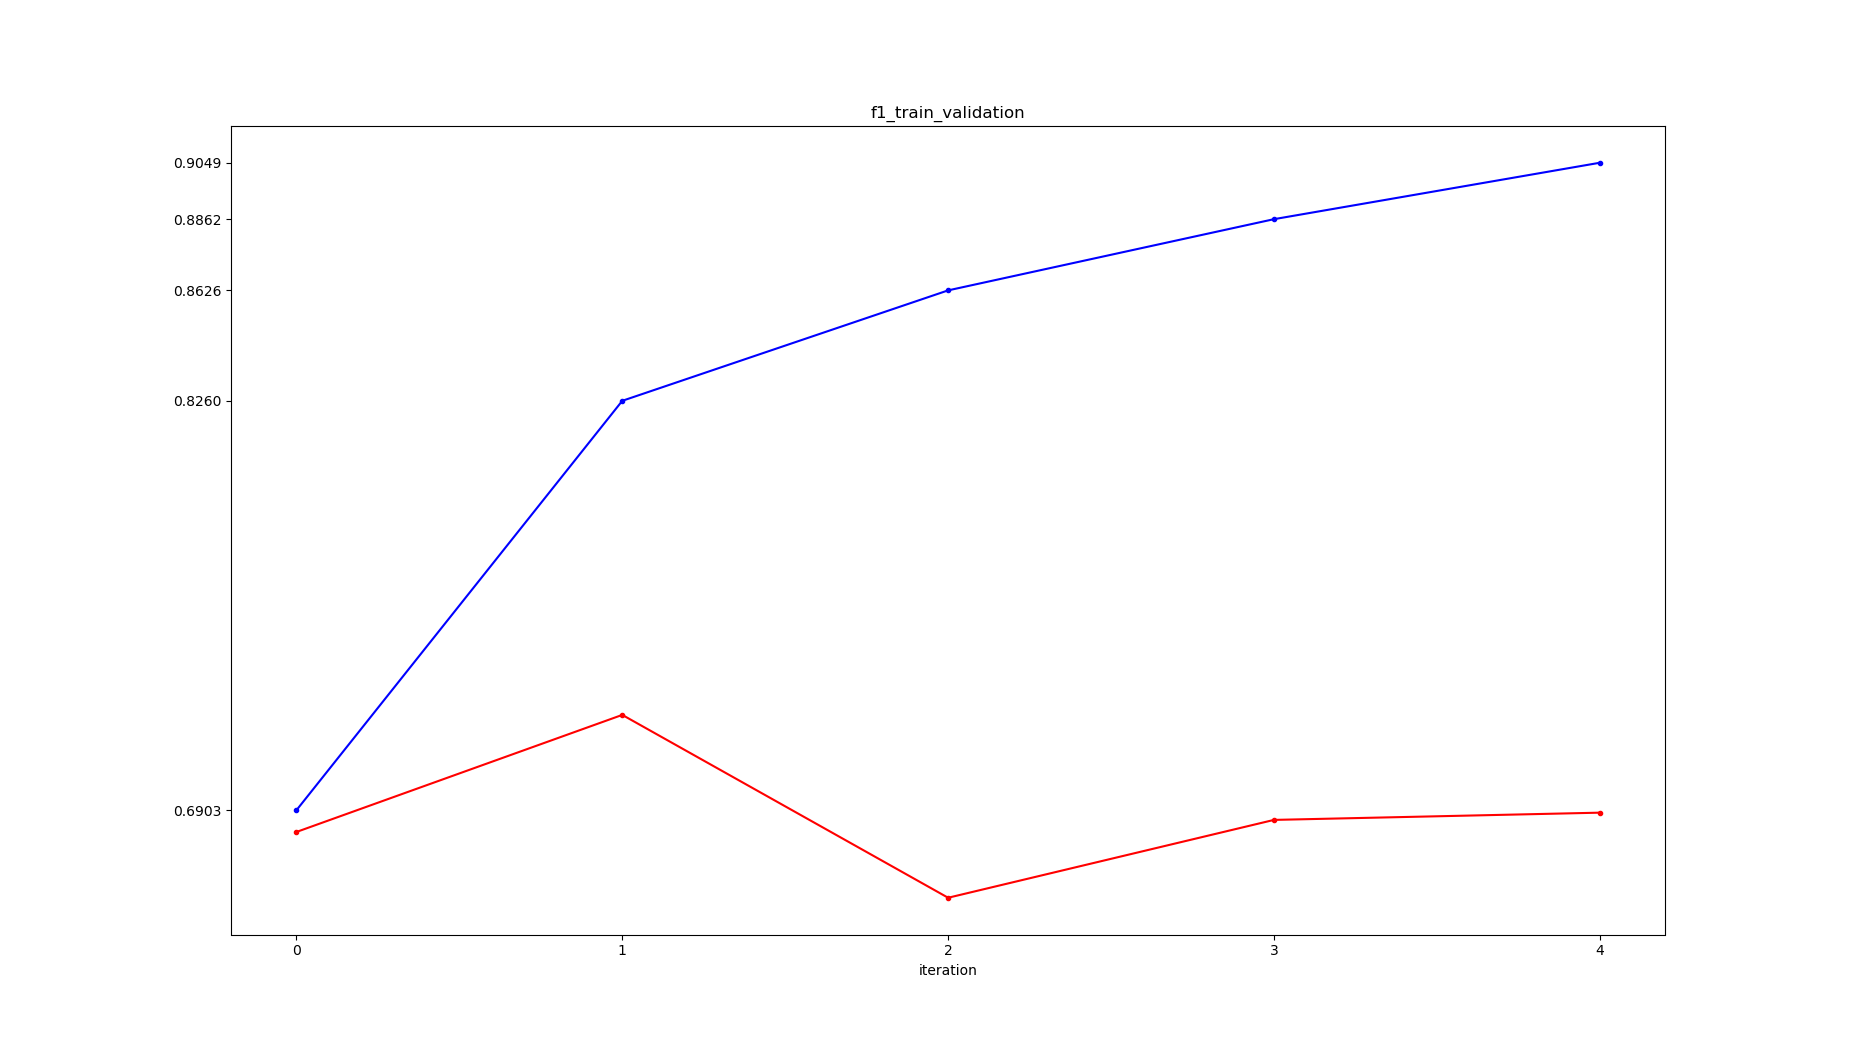
\includegraphics[width=0.5\textwidth]{images/graph_f1_train_validation.png}
    \caption{Training / Validation F1 - red validation data set, blue train data set}
    \label{fig:train_validation_f1}
\end{figure}

\section{Conclusions}
This paper presents the system developed by our group for the EmoContext task. The architecture of the system includes data processing, feature selection, and machine learning model. The results are promising, but they also expose the need for more experiments that should be done in this field in the next period.

For the future, we believe a CNN approach could prove fruitful. As well as a different or deeper network and configuration while using a similar pre-processing process which we believe is the main contributor to our relatively successful result.

Another direction worth investigating would be a Mixture of Experts approach, using various variations of the system even if they prove sub-optimal individually, such as \textit{The currently proposed system}; \textit{A system using a pre-trained embedding}; \textit{Three sub-systems each trained to only classify one of the classes}; \textit{A system with three input layers, one for each message reply, removing the concatenation of the text pre-processing}; \textit{A system which only looks at the emoticons present in the text}.

\section*{Acknowledgments}

This work is partially supported by POC-A1-A1.2.3-G-2015 program, as part of the PrivateSky project (P$\_$40$\_$371/13/01.09.2016).

% Include your own bib file like this:
% \verb|\bibliographystyle{acl_natbib}|
% \verb|\bibliography{naaclhlt2018}|
% \verb|\bibliography{naaclhlt2018}|
% Where \verb|naaclhlt2018| corresponds to a naaclhlt2018.bib file.


\bibliographystyle{acl_natbib.bst}
\bibliography{semeval2018.bib}

\nocite{*}
\printbibliography

\end{document}